% IOP Publishing journal article prepared from manuscript/main/quantum-template.tex
\documentclass{iopjournal}

\usepackage[utf8]{inputenc}
\usepackage[english]{babel}
\usepackage[T1]{fontenc}
\usepackage{amsmath,amssymb,amsfonts}
\usepackage{amsthm}
\usepackage{mathrsfs}
\usepackage{booktabs}
\usepackage{array}
\usepackage{multirow}
\usepackage{textcomp}
\usepackage{placeins}
\usepackage{xurl}

\newtheorem{theorem}{Theorem}

\begin{document}

\articletype{Paper}

\title{Risk-Aware Relational Spectral Recovery under Partial Quantum Observability}

\author{Jaeyun Jeong$^1$\orcid{0009-0005-3281-5858} and Hwa Young Jeong$^2$\orcid{0000-0002-5017-934X}}

\affil{$^1$Division of Computer Engineering, Hankuk University of Foreign Studies, 17035 Yongin, Republic of Korea}

\affil{$^2$Humanitas College, Kyung Hee University, 26, Kyungheedae-ro, 02447 Seoul, Republic of Korea}

\email{3500jjy@gmail.com; hyjeong@khu.ac.kr}

\keywords{relational spectral recovery; partial observability; quantum error correction; recovery control; spectral graph theory; quantum information; risk-aware control}

\begin{abstract}
Quantum recovery under partial observability must operate with incomplete, noisy, 
or ambiguous diagnostic evidence. In this setting, recovery policies may improve 
average logical fidelity while still introducing rare but severe lower-tail failures 
through unsafe candidate switches. We introduce a finite and auditable framework 
for risk-aware relational spectral recovery that targets this failure mode.
The method constructs internally clock-conditioned system slices and maps each 
slice to a weighted relational graph. The ordered family of graph Laplacian spectra 
defines a relational spectral representation used for admissibility-aware recovery. 
A syndrome-first candidate and a relational candidate are then evaluated by a policy 
layer. The robust controller (C_3^R) treats the balanced policy (C_2) as a proposal 
and applies a one-sided veto under excessive admissibility violation or syndrome uncertainty.
The framework is evaluated on encoded three-qubit repetition-code simulations under 
clean, partial, noisy, partial-plus-noisy, and ambiguity-driven syndrome regimes. 
The main benefit appears in the lower tail rather than in a large shift of the mean. 
In degraded regimes, (C_3^R) reduces false-safe failures and improves lower-tail recovery 
behavior while remaining inactive in clean and noisy-only negative controls. These results 
support a restricted operating-zone interpretation: the proposed framework acts as a 
conservative recovery-control layer rather than as a decoder replacement or a 
foundations-level theory of quantum time.
\end{abstract}

\section{Introduction}\label{sec:introduction}

Quantum recovery increasingly has to operate under incomplete and imperfect 
diagnostic information. In encoded quantum systems, syndrome measurements 
provide the primary evidence for selecting a correction, but this evidence 
may be missing, corrupted, ambiguous, or affected by measurement and reset errors. 
Standard recovery and mitigation frameworks address important aspects of this 
problem through recovery maps, syndrome-based correction, autonomous protection, 
probabilistic cancellation, and learning-based error mitigation~\cite{Lautenbacher2024PetzRecoveryQudit,Gertler2021AutonomousQECBosonic,VanDenBerg2023SparsePauliLindbladPEC,Strikis2021LearningBasedQEM,Liao2024MachineLearningQEM}. 
However, when observability is partial, the central issue is not only whether 
a candidate recovery improves the average logical fidelity. A policy may improve 
the mean while still producing rare but severe lower-tail failures. 
This motivates recovery criteria that explicitly account for unsafe candidate 
switches, false-safe outcomes, and uncertainty-aware intervention.
A complementary viewpoint comes from background-independent and relational formulations 
of quantum dynamics. In such settings, dynamics are not introduced by an 
externally supplied time coordinate, but are described through internal relations 
between subsystems. The Page--Wootters mechanism and related formulations show how 
clock-conditioned system states can be obtained from a constrained global state, 
providing a way to discuss internal quantum time and relational evolution~\cite{Smolin2005BackgroundIndependence,Rovelli2007QuantumGravity,Giovannetti2015QuantumTime,Marletto2017EvolutionWithoutEvolution,Hoehn2021TrinityRelationalQuantumDynamics,Rijavec2023RobustnessPageWootters}. 
In this work, we use this perspective in a deliberately narrower computational sense. 
We do not claim that a finite encoded-qubit simulation realizes a complete theory of 
quantum time. Instead, we ask whether internally clocked conditional slices can provide 
auditable evidence for recovery decisions under partial observability.
To make this evidence operational, we map each clock-conditioned system slice to a weighted 
relational graph and use the graph Laplacian spectrum as a compact structural signature. 
Spectral graph methods provide a natural way to summarize connectivity, perturbation, 
and collective structure, and prior work has connected graph Laplacians with quantum-state 
representations and quantum networks~\cite{Braunstein2006GraphLaplacianDensityMatrix,Adhikari2017WeightedDigraphsQuantumStates,Biamonte2019ComplexNetworksQuantum}. 
This motivates a relational spectral trajectory: an ordered family of Laplacian spectra 
indexed by internal clock labels rather than by an external time variable. Such a trajectory 
can be compared with reference-compatible families, audited for admissibility, and used 
to test whether a proposed recovery remains structurally consistent.
The resulting gap is between relational quantum dynamics and operational recovery control. 
Relational and Page--Wootters-type frameworks provide internally conditioned states, 
but they are rarely used as recovery-side evidence in encoded quantum systems. 
Conversely, quantum recovery, mitigation, benchmarking, and uncertainty-quantification 
methods provide tools for noisy quantum processors, but they typically operate on 
syndrome records, channel models, circuit-level characterizations, learned maps, or 
externally indexed data~\cite{Hashim2025BenchmarkingCharacterization,Bennink2026UncertaintyQuantificationQC,Cieslinski2024RandomisedMeasurements}. 
The present study connects these directions by formulating recovery as admissible 
restoration in a clock-conditioned relational spectral trajectory space.
We evaluate this framework in a controlled encoded-QEC testbed. Each simulation row 
produces two recovery candidates: a syndrome-first decoded recovery and a relational 
admissible recovery. A policy layer then decides whether a proposed switch to the 
relational candidate should be accepted or vetoed. The revised controller \(C_3^R\) 
is not designed as a universal decoder. It is a downside-risk controller that can only 
veto proposed switches from the balanced policy. This design makes the intervention 
auditable: one can ask whether the controller remains inactive in reliable regimes, 
whether it blocks harmful proposed switches under degraded syndrome evidence, and 
whether the prevented loss exceeds the missed beneficial gain.
The main contribution is therefore a finite, auditable baseline framework for 
relational spectral recovery under partial quantum observability. We define 
clock-conditioned spectral trajectories, introduce admissibility constraints 
and a reference-anchored recovery objective, and evaluate a risk-aware controller 
under clean, noisy-only, partial, partial-plus-noisy, and ambiguity-plus-measurement 
stress protocols. The results support a restricted operating-zone interpretation. 
The robust controller remains inactive in clean and noisy-only controls, but reduces 
false-safe outcomes and lower-tail fidelity failures under partial and partial-plus-noisy 
syndrome observability. Thus, the study provides evidence that relational spectral 
structure can serve as a recovery-side safety signal without claiming to replace 
optimized decoders or to establish a complete background-independent dynamics.
We present this work as the first in a planned sequence: subsequent studies will 
examine whether the same admissibility and risk-control geometry generalizes to 
nontrivial stabilizer codes, and whether the relational spectral trajectory space 
can itself be promoted from an auditable diagnostic object to a trainable structural 
representation.

\section{Background and Positioning}
\subsection{Clock-conditioned relational dynamics}

Relational formulations of quantum dynamics describe change through correlations
with an internal clock rather than an externally supplied time parameter. This
idea appears in background-independence and relational-dynamics
discussions~\cite{Smolin2005BackgroundIndependence,Rovelli2007QuantumGravity}.
The Page--Wootters mechanism gives the operational ingredient used here: a
constrained global state can be conditioned on a clock subsystem to obtain
relative system states~\cite{Giovannetti2015QuantumTime,Marletto2017EvolutionWithoutEvolution,Hoehn2021TrinityRelationalQuantumDynamics}.
Related work has studied robustness, interactions, noncausal circuits,
measurement-related time flow, and computational uses of quantum
time~\cite{Rijavec2023RobustnessPageWootters,Mendes2021NonlinearPageWootters,Baumann2022NoncausalPageWoottersCircuits,Paiva2022FlowTimeEnergyMeasurements,Diaz2025ParallelPageWoottersSimulation}.
Our use of this literature is intentionally narrow. We do not attempt to solve
the problem of time or derive continuum dynamics from a finite clock; we use
clock-conditioned slices as finite relational data objects for recovery control.

\subsection{Spectral graph representations of quantum structure}

Graph-based and spectral representations provide compact descriptions of relational 
structure. In quantum information, graph Laplacians have been related to density matrices, 
separability, and quantum-state representations~\cite{Braunstein2006GraphLaplacianDensityMatrix,Adhikari2017WeightedDigraphsQuantumStates,Bradshaw2023GraphZetaEntanglement}. 
More broadly, quantum network models provide a language for connecting graph structure, 
correlations, and quantum dynamics~\cite{Biamonte2019ComplexNetworksQuantum}. These works 
motivate the use of spectral signatures as auditable summaries of relational connectivity.

The present work differs from graph-state or network modeling approaches in its use of 
clock-conditioned spectral families. A single graph spectrum is not the central object. 
Instead, each internal clock label produces a relational graph, and the ordered family of 
Laplacian spectra defines a relational spectral trajectory. This trajectory is then compared 
with reference-compatible families and audited through admissibility penalties before it 
enters the recovery policy layer.

\subsection{Quantum recovery, mitigation, and control}
Quantum recovery and error mitigation have developed along several complementary directions. 
Recovery-map approaches formalize channel-level reconstruction and approximate reversibility~\cite{Lautenbacher2024PetzRecoveryQudit}, 
while quantum error-correction experiments and autonomous protection schemes demonstrate 
how encoded or stabilized systems can preserve quantum information under noise~\cite{Reed2013EntanglementQEC,Gertler2021AutonomousQECBosonic,Nascimento2011NoiselessSubsystem}. In the NISQ setting, mitigation methods such as probabilistic error cancellation, virtual distillation, detection-based mitigation, and learning-based correction address noisy circuit outputs without requiring full fault tolerance~\cite{VanDenBerg2023SparsePauliLindbladPEC,Xu2024CircuitNoiseResilientVirtualDistillation,Zhang2021AutoencoderErrorMitigation,Strikis2021LearningBasedQEM,Liao2024MachineLearningQEM,Liao2025NoiseAgnosticQEM}.

The proposed framework is not a replacement for these methods. It is closer 
to a recovery-control layer placed above candidate recovery mechanisms. In the 
encoded-QEC experiments, the syndrome-first recovery remains the decoder-facing 
baseline, while the relational admissible recovery supplies an alternative candidate. 
The policy layer asks when a switch to that candidate should be trusted, when it 
should be vetoed, and how the tradeoff should be evaluated under partial observability.

\subsection{Partial observability, uncertainty, and benchmarking}

Reliable recovery decisions depend on how much diagnostic information is available and 
how trustworthy that information is. Benchmarking and characterization methods provide 
tools for quantifying device behavior and validating performance claims~\cite{Hashim2025BenchmarkingCharacterization}. 
Randomized-measurement techniques and uncertainty-quantification frameworks also emphasize 
that finite, noisy, or incomplete observations must be interpreted with calibrated uncertainty~\cite{Cieslinski2024RandomisedMeasurements,Bennink2026UncertaintyQuantificationQC}. 
Noise modeling, live noise fingerprinting, robust control, and non-Markovian noise studies 
further show that quantum behavior can depend strongly on the structure and timing of noise 
processes~\cite{Ji2026DataEfficientNoiseModeling,Bensoussan2025LiveNoiseFingerprinting,Ding2025UniversallyRobustControl,Cai2020RandomTelegraphDephasing,Zhang2024NonMarkovianTeleportation,Zhuang2026FluxoniumNonMarkovian}.

The present study focuses on a narrower but related issue: unsafe candidate selection 
when syndrome evidence is partial or jointly corrupted. Rather than claiming a calibrated 
posterior uncertainty model, we use a deliberately simple syndrome-stress index and evaluate 
its behavior through threshold and uncertainty-bin diagnostics. This makes the controller 
auditable and exposes the tradeoff between preventing harmful switches and mistakenly 
blocking beneficial ones.

\section{Methods}\label{sec:methods}

This section develops the proposed framework in five steps. We first define the
background-independent clock-conditioned setting. We then construct relational
spectral signatures from each clock slice and assemble them into a spectral
trajectory. Next, we formulate recovery as admissible restoration toward a
reference-compatible spectral family. Finally, we instantiate the framework in an
encoded-QEC testbed and define the risk-aware metrics used for evaluation.
The methodological separation is important. The relational formulation specifies
where the data objects come from; the spectral representation specifies what is
measured; the recovery objective specifies how a corrupted relational trajectory is
restored; and the encoded-QEC protocol tests whether the restored trajectory should
be trusted when direct syndrome evidence is incomplete. This prevents the
controller from being interpreted as either a new universal decoder or a claim that
all clock-conditioned dynamics have been solved. The narrower claim is that
relational spectral evidence can be made auditable and can be combined with
syndrome evidence through an explicit downside-risk policy. The five-step separation 
also defines the interfaces along which subsequent work can substitute components 
without altering the surrounding decision geometry.
Figure~\ref{fig:pipeline-overview} summarizes the full pipeline, with the four numbered stages 
keyed to the subsections that follow.

\begin{figure}[t]
\centering
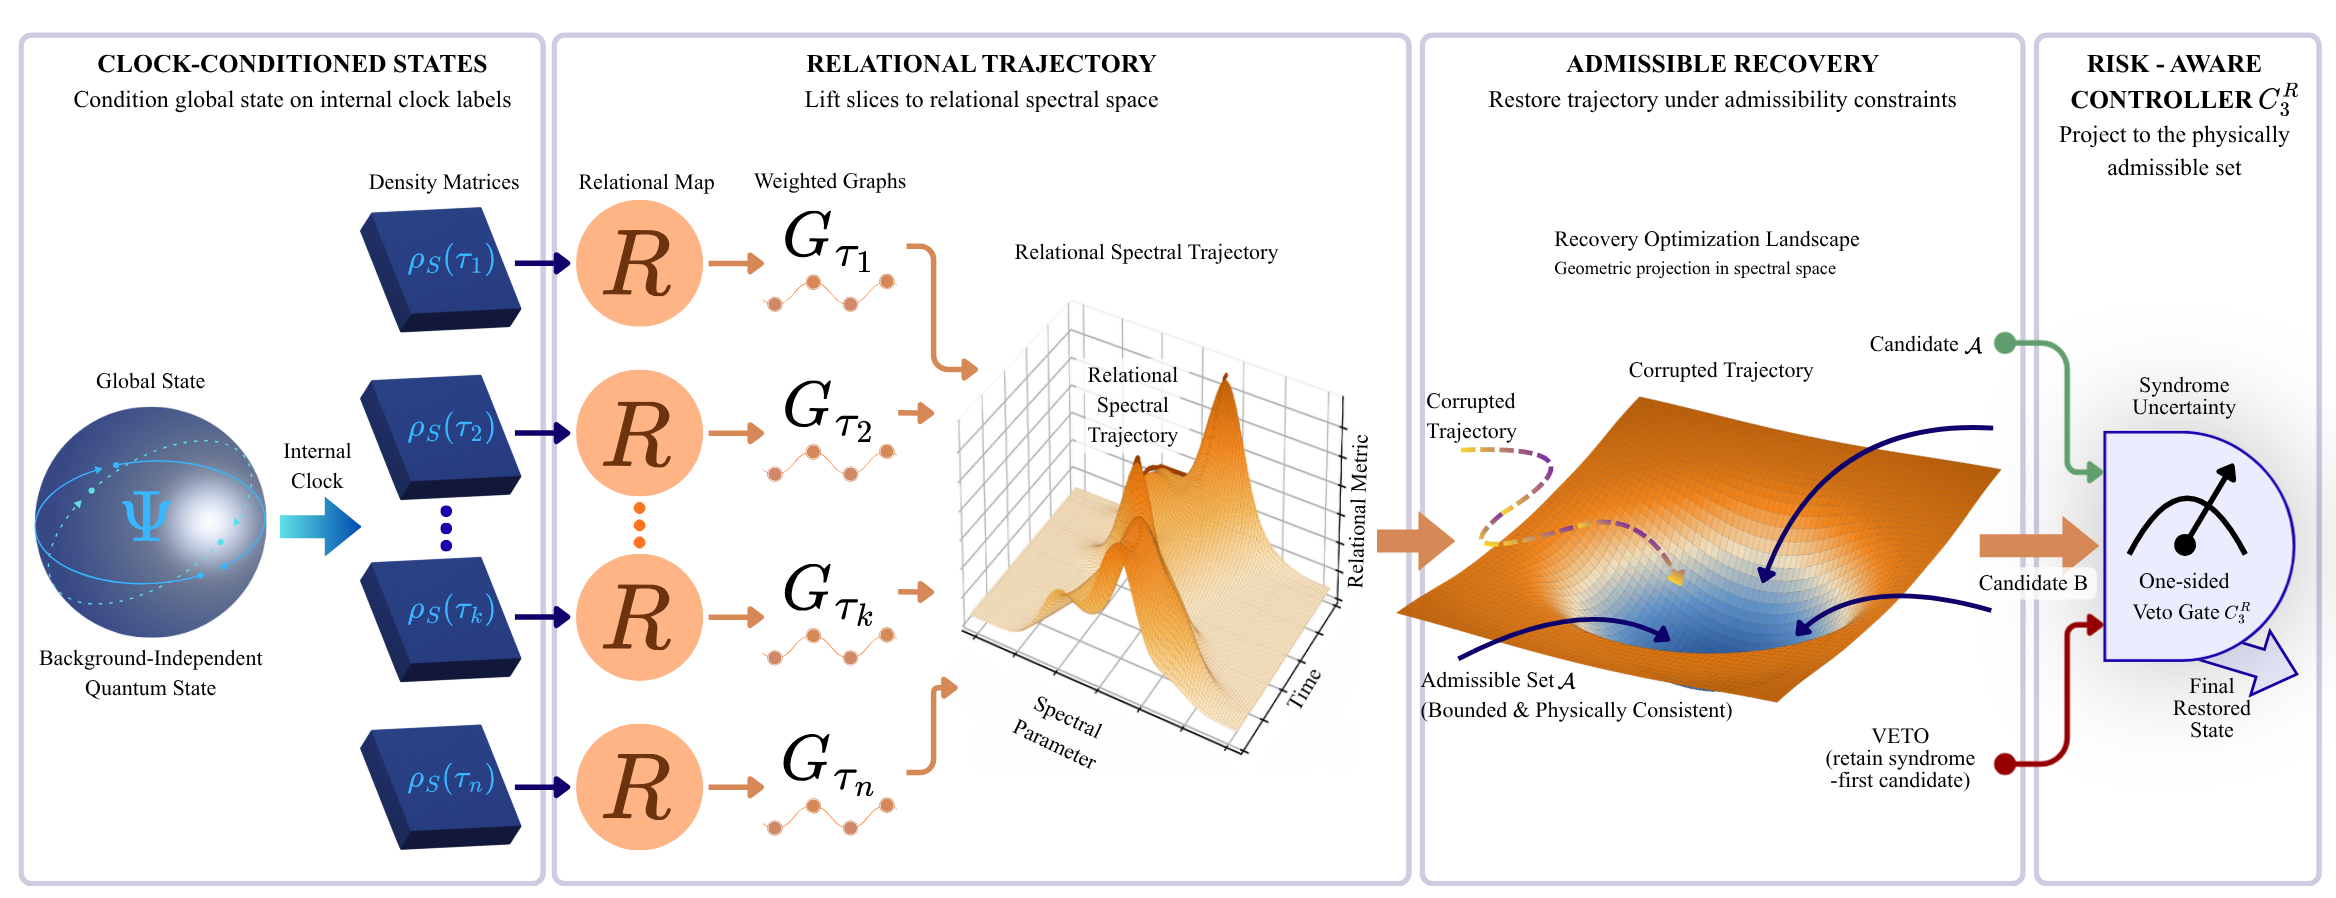
\includegraphics[width=0.95\textwidth]{main_figure.png}
\caption{Pipeline overview of the proposed framework.
A constrained global state is conditioned on internal clock labels to obtain system slices \(\rho_S(\tau_r)\).
Each slice is mapped to a weighted relational graph and reduced to a Laplacian spectral signature, yielding the relational spectral trajectory \(\Gamma_\Psi\).
The observed trajectory is restored through a reference-anchored admissible recovery objective, producing the relational candidate \(B\).
At the policy layer, \(C_3^R\) acts as a one-sided veto that can retain the syndrome-first candidate \(A\) or accept the \(C_2\)-proposed switch to \(B\).
}
\label{fig:pipeline-overview}
\end{figure}

\subsection{Clock-conditioned relational formulation}\label{subsec:relational-formulation}

We use a clock-conditioned relational formulation inspired by
background-independent quantum dynamics and relational-time
constructions~\cite{Gambini2004RelationalTime,Giovannetti2015QuantumTime,Hoehn2021TrinityRelationalQuantumDynamics}.
The total Hilbert space is decomposed as
\begin{equation}
\mathcal{H}_{\mathrm{tot}}
=
\mathcal{H}_{C}\otimes\mathcal{H}_{S},
\end{equation}
where $\mathcal{H}_{C}$ is an internal clock register and $\mathcal{H}_{S}$ is the
system register. Rather than assuming an externally supplied time coordinate, we
work with a constrained global state
\begin{equation}
\hat{H}_{\mathrm{tot}}|\Psi\rangle=0.
\end{equation}
We use this global constraint not as a claim that the finite simulation realizes a
complete Wheeler--DeWitt theory or quantum-cosmological
dynamics~\cite{Mazzitelli1992Midisuperspace,Massar1999UnitaryNonunitaryEvolution,Maki2026WheelerDeWittSolutions},
but as a construction principle for generating internally indexed conditional
system slices. In the computational pipeline, the
role of the constraint is to define the admissible clock-conditioned family
$\{\rho_S(\tau_r)\}_{r=1}^{m}$, from which all relational spectra, recovery
objectives, and policy diagnostics are derived. In a finite-dimensional
simulation, the existence and resolution of clock labels depend on spectral
matching and recurrence constraints; those conditions are treated as consistency
requirements and are moved to the Supplementary Information.

For a clock label $\tau$, the clock-conditioned system state is
\begin{equation}
\rho_S(\tau)
=
\frac{
\operatorname{Tr}_{C}\!\left[
\left(|\tau\rangle\langle\tau|_{C}\otimes I_S\right)
|\Psi\rangle\langle\Psi|
\right]
}{
\operatorname{Tr}\!\left[
\left(|\tau\rangle\langle\tau|_{C}\otimes I_S\right)
|\Psi\rangle\langle\Psi|
\right]
}.
\label{eq:clock-conditioned-state}
\end{equation}
We therefore do not model recovery as a trajectory over an externally supplied
background time coordinate. Instead, we condition a timeless global state on
internal clock labels and construct recovery evidence from the resulting
relational slices. Detailed consistency conditions for the global constraint,
finite-dimensional clock representation, and clock-resolution assumptions are
provided in Supplementary Note S1.
In the implementation, each encoded simulation instance uses one clock qubit with
initial state $|+\rangle_C$ and clock Hamiltonian $H_C=0.8X_C$. The clock grid is
uniform with
\begin{equation}
m=9,\qquad
\tau_r\in\{-2.0,-1.5,\ldots,1.5,2.0\}.
\end{equation}
The conditional states $\rho_S(\tau_r)$ are materialized from the simulated global
density matrix using Eq.~\eqref{eq:clock-conditioned-state}. Unless otherwise
stated, the same clock grid, clock Hamiltonian, and conditional-slice construction
are used for all policies and stress protocols. This finite sampling is also why
the framework is naturally compatible with partial observability: a degraded
experiment may hide or corrupt part of the evidence available to the policy layer
without changing the underlying definition of a clock-conditioned slice.
The one-qubit clock is used deliberately as a minimal finite relational clock,
not as a continuum-clock
approximation~\cite{Foti2021ClassicalEquationsPageWootters,Rijavec2023RobustnessPageWootters}.
This choice keeps the validation focused
on the minimal controlled question: whether clock-conditioned relational spectra
can provide auditable recovery evidence before scaling to larger clock registers
or denser relational clocks.

\subsection{Relational spectral representation}\label{subsec:spectral-representation}

For each clock-conditioned state $\rho_S(\tau)$, we build a weighted relational
network whose edge weights encode pairwise relational evidence between system
degrees of freedom,
\begin{equation}
\begin{aligned}
W^{(\tau)}_{ij}
&=
f(\rho_S(\tau);i,j),\\
W^{(\tau)}_{ij}
&=
W^{(\tau)}_{ji},
\qquad
W^{(\tau)}_{ij}\ge 0.
\end{aligned}
\end{equation}
The reported experiments use explicit pairwise functionals rather than leaving
$f$ unspecified. Let $\rho_{ij}^{(\tau)}$ be the two-qubit reduction of
$\rho_S(\tau)$ and let $\rho_i^{(\tau)}$ be the one-qubit reduction. For
phase-flip-code experiments we use the absolute two-qubit coherence score
\begin{equation}
W^{(\tau)}_{ij}
=
\sum_{a\ne b}
\left|(\rho_{ij}^{(\tau)})_{ab}\right|,
\qquad i\ne j,
\label{eq:coherence-weight-main}
\end{equation}
in the computational basis. For bit-flip-code experiments we use the von Neumann
mutual-information score
\begin{equation}
W^{(\tau)}_{ij}
=
S(\rho_i^{(\tau)})
+
S(\rho_j^{(\tau)})
-
S(\rho_{ij}^{(\tau)}),
\label{eq:mutual-info-weight-main}
\end{equation}
with negative numerical round-off clipped to zero. Alternative pairwise
functionals are possible and are treated as representation-robustness questions
for future work, but all reported policy comparisons use the fixed code-dependent
mapping above.
The two choices reflect the dominant relational signature of the corresponding
encoded basis. Phase-flip protection is sensitive to phase coherence, so the
computational-basis coherence functional directly measures off-diagonal
relational structure. Bit-flip protection is associated with population-basis
error structure, for which mutual information provides a basis-independent
pairwise dependence score. Because this choice can affect
sensitivity, we treat representation robustness as a limitation rather than
claiming uniqueness of the graph functional.
We use a graph Laplacian rather than raw edge weights because its
spectrum summarizes collective connectivity, is stable under node relabeling, and
allows perturbations to be compared through standard spectral
quantities~\cite{JiangSpectralGraphTheory,Braunstein2006GraphLaplacianDensityMatrix,Adhikari2017WeightedDigraphsQuantumStates}.

The corresponding degree matrix and graph Laplacian are
\begin{equation}
D^{(\tau)}_{ii}=\sum_{j\neq i} W^{(\tau)}_{ij},
\qquad
L(\tau)=D^{(\tau)}-W^{(\tau)}.
\end{equation}
Let the ordered Laplacian spectrum be
\begin{equation}
\begin{aligned}
\Lambda(\tau)
&=
\left(\lambda_1(\tau),\ldots,\lambda_n(\tau)\right),\\
\lambda_1(\tau)
&\le
\cdots
\le
\lambda_n(\tau).
\end{aligned}
\end{equation}
The central object is not an individual graph or a single spectrum, but the
clock-conditioned spectral family
\begin{equation}
\Gamma_\Psi:T\rightarrow\mathbb{R}^{n},
\qquad
\Gamma_\Psi(\tau)=\Lambda(\tau).
\label{eq:spectral-family}
\end{equation}
We use the term trajectory to denote an ordered family over internal clock labels,
not evolution with respect to external background time.
This distinction matters for the recovery task. A local perturbation at one clock
slice may be harmless if it is compatible with the neighboring slices, but the same
perturbation can be suspicious if it creates a discontinuity in the spectral
family. The object being recovered is therefore the whole clock-indexed spectral
signature, not a collection of independent spectra. This representation is
intended to expose relational inconsistencies that may not be captured by a single
syndrome snapshot.

Computationally, the collection of admissible spectral families is treated as a
constrained metric trajectory space. For two spectral families
$\Gamma^{(a)}$ and $\Gamma^{(b)}$ sampled at clock labels
$\{\tau_r\}_{r=1}^{m}$, we use
\begin{equation}
\begin{aligned}
d_{\mathcal M}^{ab}
&\equiv
d_{\mathcal{M}}\!\left(\Gamma^{(a)},\Gamma^{(b)}\right),\\
d_{\mathcal M}^{ab}
&=
\left(
\sum_{r=1}^{m}
w_r
\left\|
\Lambda^{(a)}(\tau_r)-\Lambda^{(b)}(\tau_r)
\right\|_2^2
\right)^{1/2}.
\end{aligned}
\label{eq:trajectory-distance}
\end{equation}
The manifold terminology used below should be read as a formal geometric
interpretation of this metric trajectory representation. The detailed tangent-space,
geodesic, and perturbation arguments are given in Supplementary Notes S2 and S3.
The weights $w_r$ allow the implementation to emphasize or de-emphasize particular
clock slices, but the experiments reported here use the same metric form across
all policies. Thus differences between $C_1$, $C_2$, $C_3$, and
$C_3^{\mathrm R}$ arise from the decision layer, not from changing the underlying
trajectory distance.

\subsection{Admissible spectral recovery}\label{subsec:admissible-recovery}

Let $\Gamma_{\mathrm{obs}}$ be the observed spectral trajectory after noise or
partial observation. Recovery is posed as a constrained restoration problem in
spectral-trajectory space. We define an admissible set
\begin{equation}
\mathcal{A}
=
\mathcal{A}_{\mathrm{lap}}
\cap
\mathcal{A}_{\mathrm{rel}}
\cap
\mathcal{A}_{\mathrm{ref}},
\end{equation}
where $\mathcal{A}_{\mathrm{lap}}$ enforces Laplacian spectral constraints,
$\mathcal{A}_{\mathrm{rel}}$ enforces relational smoothness and clock consistency,
and $\mathcal{A}_{\mathrm{ref}}$ constrains compatibility with a reference family.
In implementation these constraints are audited through penalty functions
$\{\Phi_k\}_{k\in\mathcal{K}}$ with calibrated thresholds $\{\theta_k\}$.
These three constraint classes play different roles. Laplacian constraints prevent
spectral objects that cannot arise from an admissible relational graph. Relational
smoothness penalizes abrupt clock-slice variation that is not supported by the
reference dynamics. Reference compatibility prevents the recovery from drifting
toward a structurally valid but physically irrelevant spectral family. We keep
these as separate penalties rather than collapsing them into a single score so
that later policy decisions can identify whether a candidate failed because of
structure, relational continuity, or reference mismatch.

In the experiments, $\Phi_{\mathrm{lap}}$ is the sum over clock slices of
structural Laplacian violations: symmetry error, positive-semidefinite violation,
row-sum violation, positive off-diagonal violation, and diagonal-consistency
error. $\Phi_{\mathrm{smooth}}$ penalizes slice-to-slice spectral jumps by summing
$\|\Lambda(\tau_{r+1})-\Lambda(\tau_r)\|_2^2/(\tau_{r+1}-\tau_r)^2$.
$\Phi_{\mathrm{clock}}$ compares spectral response between neighboring slices to
the distinguishability of the corresponding clock states, and
$\Phi_{\mathrm{ref}}$ is the squared distance to the nearest reference trajectory.
Thresholds are calibrated as $\mu+\kappa\sigma$ over the reference bank, with
$\kappa=1.5$ for the admissibility checks used in the encoded experiments.
We use $\kappa=1.5$ as a fixed operating tolerance for this baseline study; it is
not optimized per regime.

For a candidate trajectory $\Gamma_X$, the normalized admissibility violation is
\begin{equation}
v_X
:=
\max_{k\in\mathcal{K}}
\max\left\{0,
\frac{\Phi_k(\Gamma_X)-\theta_k}{\theta_k+\epsilon}
\right\}.
\label{eq:normalized-violation-main}
\end{equation}
Thus $v_X=0$ means that all active constraints are within threshold, while
positive values measure the worst normalized excursion beyond the admissible
boundary.

Admissibility defines which spectral families are physically and structurally
acceptable. It does not by itself provide a restoration direction. We therefore
introduce a reference-anchor term that explicitly pulls the recovered trajectory
toward the nearest compatible reference family. Given a reference bank
$\mathcal{R}$, the anchor is
\begin{equation}
\Gamma_{\mathrm{ref,anchor}}
=
\arg\min_{\Gamma'\in\mathcal{R}}
d_{\mathcal{M}}\!\left(\Gamma',\Gamma_{\mathrm{obs}}\right)^2.
\end{equation}
This anchor is the key distinction between feasibility and recovery. A projection
onto $\mathcal{A}$ alone could return a trajectory that is merely allowed; it need
not be the trajectory most compatible with the unperturbed relational behavior.
The reference bank supplies a local restoration direction without requiring the
method to know the clean trajectory of the test instance. In the encoded
experiments, the bank contains three clean reference trajectories per code
configuration: the corresponding logical reference state for the code
configuration and two phase-rotated logical references at $\pm20^\circ$. The bank
is generated with the same code, clock grid, clock Hamiltonian, and graph
functional as the test row, but with the noise schedule removed. For each
observed trajectory, the anchor is selected using
only $d_{\mathcal M}(\Gamma',\Gamma_{\mathrm{obs}})$; no clean logical outcome,
candidate fidelity, or row-level oracle information is used during anchor
selection.
The three-anchor bank is intentionally minimal. It tests whether a small
auditable reference family can support recovery-side control, not whether a dense
clean-state manifold has been approximated.

The recovery objective is
\begin{equation}
\begin{aligned}
J_{\mathrm{rec}}(\Gamma)
= {}&
\alpha
d_{\mathcal{M}}\!\left(\Gamma,\Gamma_{\mathrm{obs}}\right)^2
\\
&+
\beta
d_{\mathcal{M}}\!\left(\Gamma,\Gamma_{\mathrm{ref,anchor}}\right)^2
\\
&+
\lambda_1\Phi_{\mathrm{lap}}(\Gamma)
+
\lambda_2\Phi_{\mathrm{smooth}}(\Gamma)
\\
&+
\lambda_3\Phi_{\mathrm{clock}}(\Gamma).
\end{aligned}
\label{eq:recovery-objective-main}
\end{equation}
The first term keeps the recovered trajectory close to the observation, so the
method does not discard the measured evidence. The second term pulls the solution
toward the nearest compatible reference family, providing the actual restoration
direction. The penalty terms then audit whether the resulting trajectory remains
structurally and relationally admissible. This separation is deliberate: a
candidate can be close to the observation but inadmissible, admissible but pointed
toward the wrong reference family, or reference-compatible but too discontinuous
across clock labels.

In the main experiments, we use the discrete admissible projection as the default
recovery operator because it is stable, interpretable, and directly auditable.
Continuous convex refinement is treated as a diagnostic extension and reported in
the Supplementary Information. Further details on admissibility penalties,
reference-bank construction, anchor-weight calibration, and the two-stage recovery
algorithm are provided in Supplementary Note S4.

\subsection{Encoded-QEC validation protocol}\label{subsec:qec-validation}

The encoded-QEC setting is used as a controlled testbed for partial observability
and unsafe recovery transitions. We do not claim that the proposed controller
replaces optimized decoders for all QEC regimes. Instead, the testbed evaluates
whether relational evidence can safely assist recovery when syndrome information is
complete, missing, corrupted, ambiguous, or affected by measurement/reset errors.
This framing is narrower than a decoder benchmark. The purpose of the encoded-QEC
setting is to create a situation in which two plausible recovery candidates are
available and the reliability of direct syndrome evidence can be systematically
degraded. The scientific question is then not simply which candidate has the
higher average fidelity, but when a policy should refuse a relational switch
because the evidence supporting it has become unsafe.

Each simulation row produces two recovery candidates:
\begin{equation}
A := \text{syndrome-first decoded recovery},
\qquad
B := \text{relational admissible recovery}.
\end{equation}
Candidate $A$ is obtained by applying the code-specific syndrome recovery rule to
the observed quantum trajectory. Candidate $B$ is obtained by the admissible
spectral recovery objective in Eq.~\eqref{eq:recovery-objective-main}. The policy
layer then decides whether the relational candidate is sufficiently reliable to
replace the syndrome-first candidate.
Both candidates are evaluated against the same clean logical trajectory when
computing outcomes, but the policy layer does not use that clean trajectory when
making the decision. It sees only the candidate diagnostics, observed syndrome
summary, admissibility reports, recovery objective, and uncertainty proxy. This
separation is necessary because the intervention metrics later use the clean
trajectory only as offline ground truth for analysis.

The experiments use three-qubit repetition codes in bit-flip and phase-flip
configurations, with bit-flip, phase-flip, depolarizing, dephasing, and mixed-Pauli
noise families. Each reported regime cell is averaged over seeds $11$--$20$,
giving ten random seeds per cell. The output-stem suffix \texttt{seed10} is a
batch label for this ten-seed set. The encoding and syndrome-extraction circuits
for both code configurations are shown in Supplementary Figs.~S1 and~S2.
Syndrome observability is controlled by the observation ratio
$r_{\mathrm{obs}}$, syndrome-bit corruption probability $p_{\mathrm{noise}}$,
ambiguity level $a_{\mathrm{amb}}$, measurement error probability $p_{\mathrm{meas}}$,
reset error probability $p_{\mathrm{reset}}$, and measured syndrome information loss
$\ell_{\mathrm{syn}}$. These quantities define the raw and clipped uncertainty
proxies
\begin{equation}
u_{\mathrm{raw}}
=
(1-r_{\mathrm{obs}})
+p_{\mathrm{noise}}
+a_{\mathrm{amb}}
+p_{\mathrm{meas}}
+p_{\mathrm{reset}}
+\ell_{\mathrm{syn}},
\qquad
u_{\mathrm{syn}}=\mathrm{clip}_{[0,1]}(u_{\mathrm{raw}}).
\end{equation}
The uncertainty proxy is a deliberately simple additive stress index rather than a
calibrated posterior uncertainty. The clipped value is used by the decision gate
so that $u_{\max}=0.99$ implements a conservative saturation rule: saturated
uncertainty blocks a proposed relational switch, while non-saturated uncertainty
leaves the $C_2$ proposal eligible. The raw uncertainty is retained for diagnostics
and bin-wise analysis. This distinction is important in the partial-plus-noisy and
ambiguity-plus-measurement regimes, where several moderate degradations can combine
into saturated decision uncertainty.

We compare four policies on the same candidates $A$ and $B$. $C_1$ is a
rule-based conservative hybrid that switches to $B$ only when $A$ is inadmissible
and $B$ is admissible, or when $B$ is admissible, has lower recovery objective, and
the observed syndrome is consistent. $C_2$ is the balanced proposal policy
\begin{equation}
S_X^{(2)}
=
\lambda_s s_X
-\lambda_t d_X
-\lambda_i(1-a_X)
+\lambda_o\frac{1}{1+J_X},
\end{equation}
where $a_X$ is the admissibility indicator, $d_X$ is the trajectory distance to the
observed trajectory, and $s_X$ is the syndrome-support score. The current
experiments use
\begin{equation}
(\lambda_s,\lambda_t,\lambda_i,\lambda_o)=(1.0,1.0,2.0,0.5).
\end{equation}
$C_3$ is a hard-admissibility ablation: if exactly one of $A$ and $B$ is
admissible, it selects the admissible candidate; otherwise it falls back to a
safety-weighted score. The initial $C_3$ policy was designed to test whether a
globally strict safety-first region exists. Because this strict policy did not form
an independent operating zone in the regime map, we use $C_3^{\mathrm{R}}$ as the
revised risk-aware controller that preserves the safety motivation of $C_3$ while
applying intervention only to proposed $C_2$ switches.
This policy sequence is intentionally cumulative. $C_1$ represents a conservative
rule-based baseline. $C_2$ asks whether a balanced score can use relational
evidence without excessive switching. $C_3$ tests whether a strict Boolean
admissibility rule creates a distinct safety-first region. $C_3^{\mathrm R}$ is
the revised controller used by the current study: it keeps $C_2$ as the proposal
mechanism, but only allows its proposed switch to survive if additional safety and
uncertainty gates pass.

The robust policy $C_3^{\mathrm{R}}$ treats $C_2$ as a proposal and applies a
one-sided veto. Let $\Delta S=S_B^{(2)}-S_A^{(2)}$. The gate is
\begin{equation}
\begin{aligned}
C_3^{\mathrm{R}}=B
\Longleftrightarrow\;&
\left[C_2=B\right]
\\
&\wedge
\left[\Delta S\ge\delta_S\right]
\\
&\wedge
\left[v_A\ge\delta_A\right]
\\
&\wedge
\left[B\ \mathrm{admissible}\right]
\\
&\wedge
\left[v_B\le\delta_B\right]
\\
&\wedge
\left[u_{\mathrm{syn}}\le u_{\max}\right].
\end{aligned}
\label{eq:c3r-gate-main}
\end{equation}
Otherwise $C_3^{\mathrm{R}}=A$. The main operating point is
\begin{equation}
\begin{aligned}
\delta_S&=0,
\qquad
\delta_A=0,\\
\delta_B&=0,
\qquad
u_{\max}=0.99.
\end{aligned}
\end{equation}
Thus $C_3^{\mathrm{R}}$ can only block $C_2$ switches; it never creates additional
switches that $C_2$ rejected. The policy should therefore be interpreted as a
downside-risk controller rather than a fourth independently tuned score rule.
At the main operating point, the $v_A\ge\delta_A$ condition is nonrestrictive
because $v_A\ge0$ by definition. The active default gate therefore tests whether
the $C_2$-proposed relational candidate is score-supported, exactly admissible
within the calibrated tolerances, and not exposed to saturated syndrome
uncertainty. We keep the $v_A$ term in Eq.~\eqref{eq:c3r-gate-main} because it is
part of the general gate family and can be activated in ablations.
At this operating point, the uncertainty gate is the dominant veto mechanism in
saturated-stress rows, while the exact-admissibility condition prevents accepting
relational candidates that already violate the calibrated admissible set.
Complete policy maps, decision reasons, and operating-zone summaries are provided in
Supplementary Notes S5 and S6.
The clean-regime role of $C_3^{\mathrm R}$ is correspondingly limited. If syndrome
evidence is reliable and the uncertainty gate is open, the robust policy should
often reduce to $C_2$. Its value is tested primarily in regimes where syndrome
evidence is partial, corrupted, or ambiguous enough that a proposed relational
switch carries elevated downside risk.

\subsection{Evaluation metrics and operating criteria}\label{subsec:evaluation-metrics}

Since the controller is designed to suppress unsafe recovery transitions rather than
maximize average fidelity alone, we evaluate both central performance and
lower-tail risk. For each policy $C$, let
\begin{equation}
\Delta F_C=F_C-F_{\mathrm{before}}
\end{equation}
be the logical-fidelity gain relative to the noisy observed trajectory before
recovery. Central performance is summarized by the mean gain
$\overline{\Delta F}_C$, the logical-success rate
$P(F_C\ge F_{\mathrm{success}})$, and the non-worsening rate
$P(\Delta F_C\ge0)$.
Unless otherwise stated, all reported comparisons use
\begin{equation}
\varepsilon_F=0.01,\qquad F_{\mathrm{success}}=0.99.
\end{equation}
These thresholds are fixed before policy comparison and are not tuned per regime.
Mean gain alone is not sufficient for this study. A policy could improve the mean
by taking aggressive relational switches while still creating rare but severe
regressions. Because the controller is intended to regulate unsafe transitions, we
require metrics that expose the lower tail of the gain distribution and the
quality of the blocks performed by $C_3^{\mathrm R}$.

Downside risk is summarized by the fidelity false-safe rate
\begin{equation}
\mathrm{FS}_F(C)
=
P\!\left[\Delta F_C<-\varepsilon_F\right],
\end{equation}
the empirical lower quantile $q_{0.05}(C)$, and the lower conditional value at risk
\begin{equation}
\mathrm{CVaR}_{0.05}(C)
=
\widehat{\mathbb{E}}
\left[
\Delta F_C\mid \Delta F_C\le q_{0.05}(C)
\right].
\end{equation}
A successful risk controller should remain inactive when syndrome evidence is
reliable, but should reduce false-safe and lower-tail failures under partial
observability.
We also use oracle regret as an offline diagnostic. For each row, define
\begin{equation}
\begin{aligned}
\Delta F^\star
&=
\max\{\Delta F_A,\Delta F_B\},\\
\mathrm{Reg}(C)
&=
\Delta F^\star-\Delta F_C.
\end{aligned}
\end{equation}
This quantity does not define an implementable policy because it uses the
row-level best candidate after the fact. It is nevertheless useful for measuring
how far a policy falls from the best available candidate in the two-candidate
decision problem.

For $C_3^{\mathrm{R}}$, we additionally evaluate the quality of its interventions
against the $C_2$ proposal. The block indicator is
\begin{equation}
B_R=\mathbf{1}[C_2=B]\mathbf{1}[C_3^{\mathrm{R}}=A].
\end{equation}
A proposed $C_2$ switch is called harmful when
\begin{equation}
H_2
=
\mathbf{1}[C_2=B]
\mathbf{1}[\Delta F_A>\Delta F_B+\varepsilon_F],
\end{equation}
and beneficial when
\begin{equation}
G_2
=
\mathbf{1}[C_2=B]
\mathbf{1}[\Delta F_B>\Delta F_A+\varepsilon_F].
\end{equation}
We report the block rate $P(B_R=1\mid C_2=B)$, harmful-block precision
$P(H_2=1\mid B_R=1)$, harmful-switch recall $P(B_R=1\mid H_2=1)$, and
beneficial-switch retention $P(B_R=0\mid G_2=1)$. The utility balance is
\begin{equation}
G_{\mathrm{net}}
=
\sum_i B_R^{(i)}
\max\{0,\Delta F_A^{(i)}-\Delta F_B^{(i)}\}
-
\sum_i B_R^{(i)}
\max\{0,\Delta F_B^{(i)}-\Delta F_A^{(i)}\}.
\end{equation}
Positive $G_{\mathrm{net}}$ means that, on the sampled grid, prevented harmful-switch
losses outweighed missed beneficial-switch gains. It is a sample-level intervention
diagnostic, not a theorem of dominance. We therefore also report normalized
versions, including net effect per blocked switch and per $C_2$-proposed switch,
in the Supplementary Information. Full metric definitions are given in
Supplementary Note S7, and uncertainty-threshold diagnostics are given in
Supplementary Note S8.
The final operating criterion is therefore qualitative as well as quantitative:
$C_3^{\mathrm R}$ should leave reliable regimes nearly unchanged, block a
substantial fraction of harmful $C_2$ switches under degraded syndrome evidence,
and maintain a positive net intervention balance after accounting for beneficial
switches that it mistakenly blocks.

\FloatBarrier

\section{Results}\label{sec:results}

The results support an operating-zone interpretation rather than a universal
performance claim. The relational controller is not beneficial in every regime.
Its advantage appears specifically when syndrome observability is partial or jointly
corrupted, where it suppresses unsafe recovery transitions and improves lower-tail
fidelity risk. We therefore present the results by regime and intervention
behavior, rather than ranking policies only by mean fidelity gain.

\subsection{Operating-zone structure of the baseline policies}\label{subsec:results-operating-zones}

We first evaluated the clean-syndrome regime map to determine whether the baseline
hybrid policies define distinct operating zones. The clean map contains 240
regime cells, each averaged over ten random seeds. As summarized in
Table~\ref{tab:operating-zone-summary}, $C_1$ is the preferred policy in most
cells, while $C_2$ occupies a smaller but structured correction zone. The strict
$C_3$ policy does not form an independent preferred region.

\begin{table}[t]
\caption{Baseline policy operating-zone summary under reliable syndrome evidence.
Preferred-policy counts are computed over 240 clean regime cells, with ten random
seeds per cell.}
\label{tab:operating-zone-summary}
\centering
\scriptsize
\setlength{\tabcolsep}{5pt}
\begin{tabular}{@{}lrr@{}}
\toprule
Policy & Cells & Share \\
\midrule
$C_1$ & 197 & 0.8208 \\
$C_2$ & 43 & 0.1792 \\
$C_3$ & 0 & 0.0000 \\
$C_3^{\mathrm R}$ & 0 & 0.0000 \\
\bottomrule
\end{tabular}
\end{table}

This baseline structure motivates the revised controller. The absence of a
$C_3$-dominant region does not mean that safety is irrelevant; it indicates that a
globally hard admissibility veto is too coarse for this regime map. The redesign
therefore shifts from a strict safety-first selector to $C_3^{\mathrm R}$, an
uncertainty-conditioned veto applied only to proposed $C_2$ switches.
The $C_2$-preferred cells are localized to phase-flip-code rows, with 16
dephasing, 10 phase-flip, 9 mixed-Pauli, 6 depolarizing, and 2 bit-flip cells.
We use the clean map only to identify whether the original policy family contains
distinct baseline operating zones. Degraded-regime behavior is evaluated
separately through the $C_2$ versus $C_3^{\mathrm R}$ comparison below.

\FloatBarrier

\subsection{Regime-level effect of \texorpdfstring{$C_3^{\mathrm R}$}{C3R}}\label{subsec:results-regime-effect}

The regime-level comparison between $C_2$ and $C_3^{\mathrm R}$ is shown in
Table~\ref{tab:c2-c3r-regime-metrics}. The most important pattern is selectivity:
$C_3^{\mathrm R}$ remains inactive in the clean and noisy-only controls, but
intervenes in partial and partial-plus-noisy syndrome regimes.

\begin{table}[t]
\caption{Regime-level comparison between $C_2$ and $C_3^{\mathrm R}$. Each entry
is reported as $C_2/C_3^{\mathrm R}$. Lower false-safe rate, larger $q_{0.05}$,
and larger CVaR indicate improved downside-risk behavior.}
\label{tab:c2-c3r-regime-metrics}
\centering
\tiny
\setlength{\tabcolsep}{1.5pt}
\begin{tabular}{@{}lcccccc@{}}
\toprule
Regime & Mean & Success & Non-wors. & $\mathrm{FS}_F$ &
$q_{0.05}$ & CVaR$_{0.05}$ \\
\midrule
Clean &
0.1273/0.1273 & 0.6358/0.6358 & 0.9554/0.9554 &
0.0238/0.0238 & 0.0000/0.0000 & -0.0033/-0.0033 \\
Noisy-only &
0.1169/0.1169 & 0.4556/0.4556 & 0.8814/0.8814 &
0.0678/0.0678 & -0.0104/-0.0104 & -0.0207/-0.0207 \\
Partial &
0.1169/0.1189 & 0.4552/0.5976 & 0.8774/0.9306 &
0.0694/0.0389 & -0.0152/-0.0006 & -0.0208/-0.0147 \\
Partial+noisy &
0.1170/0.1212 & 0.4551/0.7241 & 0.8792/0.9755 &
0.0685/0.0134 & -0.0104/0.0000 & -0.0206/-0.0034 \\
Ambig.+meas. &
0.1600/0.1604 & 0.5208/0.5978 & 1.0000/1.0000 &
0.0000/0.0000 & 0.0192/0.0238 & 0.0078/0.0084 \\
\bottomrule
\end{tabular}
\end{table}

In the clean map, $C_3^{\mathrm R}$ leaves the $C_2$ behavior unchanged. The
controller blocks none of the 1529 rows where $C_2$ selected the relational
candidate. In the noisy-only map, it also remains inactive: $C_2$ and
$C_3^{\mathrm R}$ have identical false-safe rate, lower-tail metrics, and logical
success rate. This provides a negative control. The robust controller does not
treat syndrome-bit corruption without observation loss as sufficient reason to
impose a universal conservative bias.
The noisy-only regime is not risk-free; its false-safe rate remains comparable to
the partial regimes. However, because the observation ratio is not reduced and the
uncertainty index does not saturate, $C_3^{\mathrm R}$ does not activate. This
clarifies that the default controller is targeted to saturated
partial-observability stress rather than to all forms of recovery risk.

\FloatBarrier

\subsection{Downside-risk reduction under partial syndrome observability}
\label{subsec:results-downside-risk}

The main benefit of $C_3^{\mathrm R}$ appears in the lower tail rather than in a
large shift of the mean. In the partial-syndrome regime, the mean gain changes
modestly from 0.1169 to 0.1189, while the false-safe fidelity rate decreases from
0.0694 under $C_2$ to 0.0389 under $C_3^{\mathrm R}$. The lower 5\% quantile moves
from -0.0152 to -0.0006, while $\mathrm{CVaR}_{0.05}$ improves from -0.0208 to
-0.0147. The logical-success rate increases from 0.4552 to 0.5976, and the
non-worsening rate increases from 0.8774 to 0.9306.

The effect is stronger under partial-plus-noisy syndrome observability. There,
$C_3^{\mathrm R}$ changes the mean gain from 0.1170 to 0.1212, but reduces the
false-safe fidelity rate from 0.0685 to 0.0134 and shifts $q_{0.05}$ from -0.0104
to 0.0000. The lower-tail $\mathrm{CVaR}_{0.05}$ improves from -0.0206 to -0.0034.
Thus the controller does not primarily act by maximizing average gain; it
suppresses the negative tail of the recovery outcome distribution. This pattern is visualized in
Fig.~\ref{fig:c3r-downside-risk}.
The reduction should be interpreted together with the uncertainty-bin analysis in
Supplementary Note S8: most blocks occur in saturated-stress rows, so the observed
lower-tail improvement reflects a conservative veto of $C_2$ switches under high
partial-observability stress.
The relational component remains essential because the veto is applied only to
$C_2$-proposed switches into the relational candidate and is conditioned on the
admissibility of that candidate.

\begin{figure}[t]
\centering
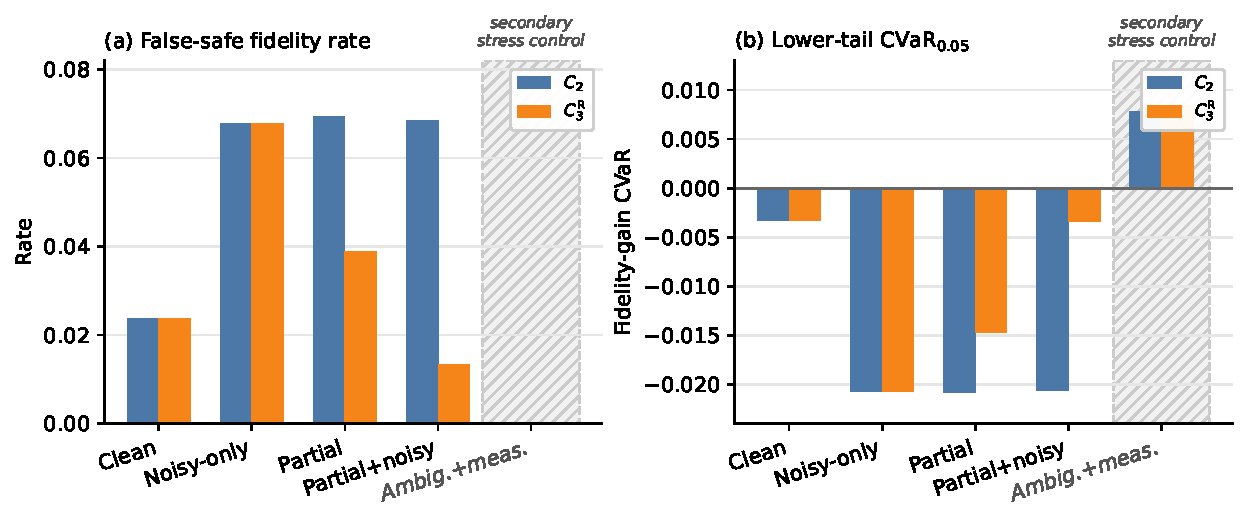
\includegraphics[width=0.95\textwidth]{c3r_downside_risk.pdf}
\caption{Downside-risk behavior of $C_2$ and $C_3^{\mathrm R}$ across syndrome
regimes. Panel~(a) shows the false-safe fidelity rate $\mathrm{FS}_F$. 
Panel~(b) shows the lower-tail fidelity-gain $\mathrm{CVaR}_{0.05}$. 
The robust controller is inactive in clean and noisy-only controls, but reduces
false-safe fidelity failures and improves lower-tail CVaR in partial and
partial-plus-noisy regimes. The ambiguity-plus-measurement regime, hatched on the right, 
is included as a secondary stress control.}
\label{fig:c3r-downside-risk}
\end{figure}

The ambiguity-plus-measurement regime is informative for a different reason. Both
$C_2$ and $C_3^{\mathrm R}$ have zero false-safe fidelity rate in this regime, so
the binary false-safe metric alone would miss any distinction. The lower-tail
metrics and logical-success rate nevertheless improve slightly under
$C_3^{\mathrm R}$, indicating that false-safe rate should be interpreted together
with lower-tail and intervention diagnostics.

\subsection{Intervention quality: harmful blocks, missed gains, and net effect}
\label{subsec:results-intervention-quality}

The previous subsection shows that $C_3^{\mathrm R}$ improves downside-risk
metrics under partial observability. We next ask why. Because $C_3^{\mathrm R}$
can only veto proposed $C_2$ switches to $B$, the relevant quantities are
conditional on $C_2=B$.

In the partial-syndrome regime, $C_2$ selected $B$ in 1094 rows and
$C_3^{\mathrm R}$ blocked 476 of those switches, a conditional block rate of
0.4351. Among the blocked switches, the harmful-block precision was 0.8697: most
blocked switches were cases where staying with $A$ would have produced larger
fidelity gain than switching to $B$. The prevented loss was 12.2670, while the
missed beneficial gain was 6.6055, yielding a positive net intervention effect of
5.6616.

In the partial-plus-noisy regime, the intervention is stronger. $C_3^{\mathrm R}$
blocked 670 of 821 proposed $C_2$ switches to $B$, with harmful-block precision
0.8791 and harmful-switch recall 0.8475. The prevented loss was 17.4350 and the
missed gain was 8.3139, giving a net intervention effect of 9.1212. This shows
that the controller is not merely blocking more transitions. It blocks harmful
transitions with high precision, and the prevented harmful loss exceeds the missed
beneficial gain. The conditional intervention rates, aggregate balance, and 
normalized net effect across the active regimes are summarized in 
Fig.~\ref{fig:c3r-intervention-quality}.

\begin{figure}[t]
\centering
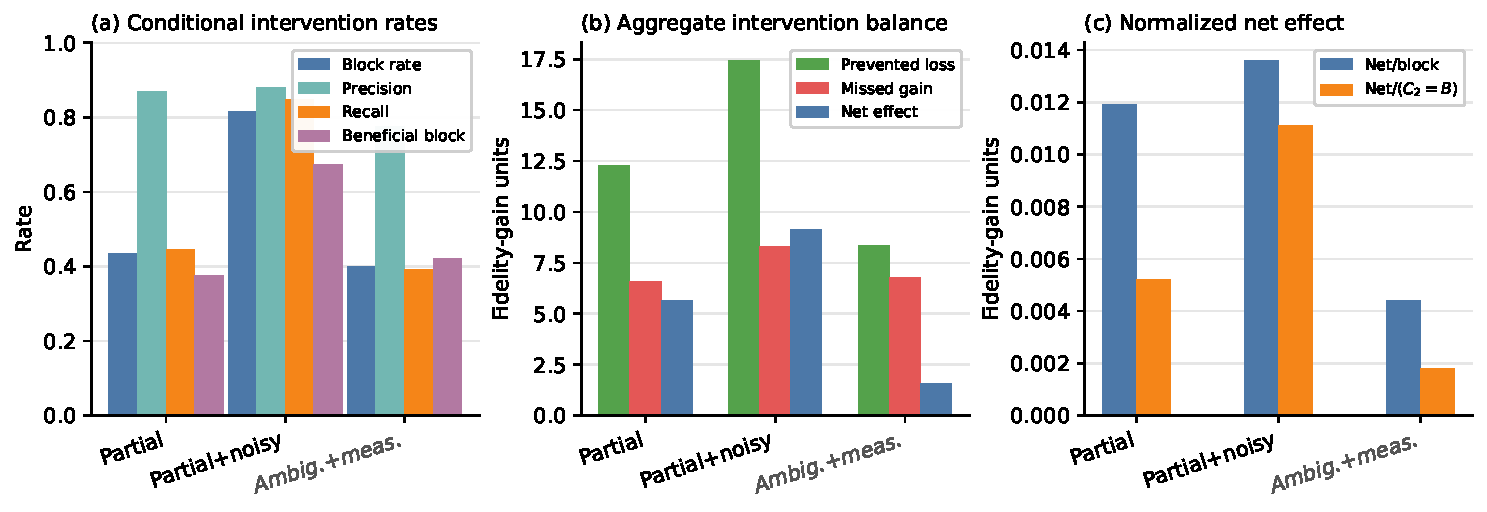
\includegraphics[width=0.95\textwidth]{c3r_intervention_quality.pdf}
\caption{Intervention quality of $C_3^{\mathrm R}$ in regimes where it actively
blocks $C_2$ switches. Panel~(a) reports the conditional intervention rates: 
block rate (given $C_2=B$), harmful-block precision, harmful-switch recall, 
and beneficial-switch block rate. Panel~(b) shows the aggregate intervention 
balance, comparing prevented harmful-switch loss, missed beneficial-switch 
gain, and the resulting net effect, all in fidelity-gain units. Panel~(c) 
normalizes the net effect per blocked switch and per $C_2$-proposed switch 
to separate aggregate benefit from the number of vetoed proposals. The 
ambiguity-plus-measurement regime is hatched as a secondary stress control.}
\label{fig:c3r-intervention-quality}
\end{figure}

The cost of the controller is also visible. $C_3^{\mathrm R}$ blocks some
beneficial switches: the beneficial-switch block rate is 0.3750 in the partial
regime, 0.6739 in the partial-plus-noisy regime, and 0.4211 in the
ambiguity-plus-measurement regime. The observed benefit therefore should not be
described as free improvement. It is a risk-control tradeoff in which missed gains
are accepted only when the prevented losses are larger on the sampled grid.
The high beneficial-switch block rate in the partial-plus-noisy regime shows that
$C_3^{\mathrm R}$ is not an efficiency-maximizing selector. Its operating point is
intentionally conservative and should be evaluated by net downside-risk reduction,
including normalized net effect, rather than by switch acceptance alone.
This cost is substantial in the partial-plus-noisy regime, where more than half
of beneficial $C_2$ switches are also vetoed. The present operating point should
therefore be viewed as a safety-biased baseline rather than a tuned optimal
controller.

\subsection{Negative controls and observed operating limits}
\label{subsec:results-limitations}

The clean and noisy-only regimes serve as negative controls. In both cases,
$C_3^{\mathrm R}$ is effectively inactive and does not materially change the
$C_2$ outcomes. This is desirable: a risk-aware controller should not impose a
universal conservative bias when the syndrome evidence is either reliable or only
mildly corrupted without partial observability. The raw uncertainty mean is 0 in
the clean map and 0.038 in the noisy-only map, far below the saturation condition
that triggers uncertainty-based veto behavior.

The strongest observed operating zone is partial-plus-noisy syndrome
observability, followed by partial syndrome observability. The
ambiguity-plus-measurement regime provides weaker but consistent supporting
evidence: $C_3^{\mathrm R}$ improves logical-success rate from 0.5208 to 0.5978
and yields positive net intervention gain, but the binary false-safe rate is
already zero for both policies. These results should not be interpreted as a
universal advantage of relational recovery over syndrome decoding. Rather, they
identify a restricted but meaningful operating zone in which relational spectral
evidence acts as a recovery-side safety signal under partial observability.
Threshold diagnostics further show that setting $u_{\max}=1.00$ removes the veto
and recovers $C_2$ behavior, whereas stricter $u_{\max}=0.75$ increases blocking
and can reduce $\mathrm{FS}_F$ further at the cost of more beneficial-switch loss.
In some regimes this becomes overly conservative. Thus the default point is not
claimed to be optimal; it is a conservative operating point that exposes the
downside-risk tradeoff.

\section{Discussion}\label{sec:discussion}

\subsection{Operating-zone interpretation of relational recovery}
\label{subsec:discussion-operating-zone}

The results support an operating-zone interpretation rather than a universal
dominance claim for relational recovery. Relational spectral evidence is useful in
the tested setting when syndrome information is sufficiently incomplete to make
some $C_2$ switches unsafe, but not so uninformative that the relational
trajectory ceases to provide a meaningful consistency signal. This explains why
$C_3^{\mathrm R}$ is inactive in clean and noisy-only controls, yet changes the
lower tail in partial and partial-plus-noisy regimes.
The roles of the two components should be separated. The relational trajectory
supplies candidate $B$, admissibility status, and trajectory diagnostics. The
uncertainty gate determines when a $C_2$-proposed use of that candidate is too
risky to accept.

The negative strict-$C_3$ result is part of this interpretation. A hard
admissibility rule does not create an independent preferred zone under reliable
syndrome evidence. Safety therefore cannot be reduced to selecting the uniquely
admissible candidate. The revised controller uses a narrower principle: keep the
balanced $C_2$ proposal mechanism, but veto proposed relational switches when the
proposal sits in a high-risk part of the policy evidence space. The main claim is
therefore not that $C_3^{\mathrm R}$ is a better decoder, but that it is a
risk-aware controller for candidate selection under partial observability.
Read as part of the baseline contribution, this negative ablation also serves a 
constructive purpose: it establishes that relational spectral evidence cannot be 
collapsed into a simpler Boolean admissibility check, which justifies the more 
elaborate one-sided veto structure that the present work and its planned 
follow-ups build on.

\subsection{Partial observability and decision geometry}
\label{subsec:discussion-partial-observability}

The relevant geometry is the geometry of the decision variables seen by the
policy. Each row supplies a score difference, admissibility status, normalized
constraint violations, and an additive syndrome-stress index. In clean regimes,
direct syndrome support keeps the $C_2$ proposal away from the veto boundary. In
noisy-only regimes, bit-level syndrome noise changes some scores but does not
produce the saturated uncertainty pattern that activates the robust gate. Partial
observability is different: the score can favor the relational candidate while the
same row has weak syndrome support and elevated uncertainty.

This is the failure mode targeted by $C_3^{\mathrm R}$. The controller does not
penalize all relational switches, and it does not treat all noise as equivalent.
It acts only after $C_2$ proposes $B$, and then requires score support,
admissible $B$, non-saturated uncertainty, and the configured violation gate. At
the default setting $\delta_A=0$, the active requirements reduce primarily to a
score-supported $C_2$ proposal, exact admissibility of $B$, and the uncertainty
saturation guard. This makes the downside-risk policy mathematically one-sided:
it can remove candidate-$B$ switches from the $C_2$ decision set, but it cannot
create new relational switches.

The intervention metrics show the cost of this one-sided geometry. Some
beneficial switches are blocked, especially in the active degraded regimes. The
reason the policy remains useful in these experiments is that the prevented
harmful-switch loss exceeds the missed beneficial gain, and this effect appears
most clearly in the lower-tail metrics. The conclusion should remain conservative:
the present evidence supports a downside-risk reduction mechanism on the sampled
grids, not a proof that the same fixed gate is optimal across codes or noise
models, nor that saturated uncertainty is the only useful trigger.

\subsection{Recovery control rather than decoder replacement}
\label{subsec:discussion-recovery-control}

The QEC role of the method is a recovery-control layer above candidate recovery
mechanisms. Candidate $A$ is the syndrome-first recovery, candidate $B$ is the
relational admissible recovery, and the policy selects between them using
diagnostics that are available before the logical outcome is evaluated. This is a
different task from constructing an optimized syndrome decoder.

This distinction sets the correct benchmark for the present study. Mean fidelity
alone is insufficient because the controller is designed to alter the lower tail
of candidate selection, not to maximize every row independently. The relevant
questions are whether reliable regimes remain nearly unchanged, whether harmful
$C_2$ switches are selectively vetoed under degraded syndrome evidence, and
whether the missed beneficial switches are smaller than the prevented losses. The
current results answer these questions for the controlled two-candidate setting.
Comparisons with optimized decoders and multi-candidate recovery sets remain
future work.
A fair next benchmark should compare not only final logical fidelity, but also
false-safe rate, lower-tail gain, and intervention regret under matched
partial-observability protocols.

The two-candidate restriction is itself a deliberate baseline choice rather 
than a structural limitation of the framework. The decision geometry of a 
one-sided veto is most clearly characterized when only one alternative to the 
syndrome-first candidate is available: the conditional metrics in 
Section~\ref{subsec:results-intervention-quality}, including block rate, 
harmful-block precision, and beneficial-switch retention, are well defined 
exactly because the policy maps a binary choice. Extending to a multi-candidate 
recovery set replaces these binary diagnostics with class-conditional analogues 
but does not alter the underlying veto principle, which acts on the 
$C_2$-proposed switch regardless of how many alternatives the proposal layer 
considers. We therefore treat $A/B$ as the smallest setting in which the 
intervention quality of $C_3^{\mathrm R}$ can be cleanly read off, and leave 
multi-candidate extension to subsequent work.

\subsection{Background-independent interpretation and spectral geometry}
\label{subsec:discussion-background-independent}

The background-independent component enters as a data-object construction. The 
global constraint motivates clock-conditioned system slices, and those slices are 
converted into relational graph spectra. The policy never uses an external 
time-indexed trajectory; it uses an ordered family of internally clocked spectral 
objects and calibrated admissibility penalties. The conceptual significance is that 
the recovery evidence is indexed by internal relational labels rather than by an 
externally supplied trajectory variable, which is what allows admissibility, 
smoothness, and clock-consistency penalties to be defined in a single relational 
language.

Operationally, the Page--Wootters-type construction is used here as a finite 
data-object construction rather than as a foundations-level theory of quantum 
time. The spectral manifold language denotes a constrained finite trajectory 
space equipped with a metric, a reference bank, and admissibility tests. That 
much is sufficient to produce a recovery-side signal: a proposed candidate can 
be checked for compatibility with clock-conditioned relational structure, and 
the resulting decision is auditable row by row. We retain the relational 
framing not because it is necessary for the present numerical experiments in 
isolation, but because it gives a structured component interface --- 
clock register, conditional slice, graph functional, spectral trajectory, 
reference bank, admissibility penalty --- along which subsequent work can 
substitute richer relational representations or learned structural maps 
without disturbing the surrounding decision geometry. In this sense the 
background-independent layer is the methodological foundation of the planned 
follow-up program rather than a self-contained claim about quantum time.

\subsection{Limitations and outlook}
\label{subsec:discussion-limitations}

We organize remaining limitations as three follow-up tracks, each of 
which corresponds to a separate planned study. The first track is QEC 
benchmarking: larger codes, broader channel families, optimized 
syndrome decoders, and multi-candidate recovery sets are needed before 
making stronger decoder-level 
claims~\cite{Asaka2026QuantumSpatialQEC,Filippov2024ScalabilityErrorMitigation,Li2025ZMixedAmplitudeDamping}. 
The present work establishes a controlled baseline for two-candidate 
selection, not a competitive decoder benchmark, and the result also 
depends on the two-candidate formulation $A/B$; a larger candidate set 
may change the intervention tradeoff. Whether the same operating-zone 
and downside-risk geometry persist when the relational signal is 
applied to nontrivial stabilizer codes such as the $[[5,1,3]]$ perfect 
code, the Steane code, and the Shor nine-qubit code is the subject of 
forthcoming work.

The second track is relational representation. The graph functional is fixed in
the reported experiments, with mutual information used for the bit-flip code and
absolute two-qubit coherence used for the phase-flip code. Alternative
functionals, larger reference banks, multipartite relational witnesses, and learned
relational summaries may change the sensitivity of the spectral trajectory and
should be tested
explicitly~\cite{Brito2020MultipartiteInterference,Huang2026QuantumSpectralPDEs,Alexeev2025AIQuantumComputing}.

The third track is uncertainty and control. The current uncertainty proxy is an
additive stress index, not a calibrated posterior. The default
$u_{\max}=0.99$ gate is best interpreted as a saturation guard, and the
normalized intervention metrics show that the gate trades missed beneficial
switches against prevented harmful switches. Future work should calibrate this
uncertainty more directly, learn adaptive thresholds, and test whether the same
downside-risk geometry persists beyond the sampled regimes and under pulse- or
control-level optimization constraints~\cite{Mohseni2021AdiabaticErrorSuppression,Lewis2026PulseQualityOptimisation}.
We also stress-tested the admissibility threshold itself by varying 
$\kappa\in\{1.0,1.5,2.0\}$ across a balanced grid of $135$ recovery cases 
(see Supplementary Note~S8): admissibility coverage saturates at 
$\kappa=1.5$ and remains stable up to $\kappa=2.0$, while $\kappa=1.0$ 
leaves most recovered trajectories outside the calibrated admissible set. 
The default $\kappa=1.5$ should therefore be read as the smallest tolerance 
at which admissibility coverage saturates on the sampled configurations, 
not as a tuned optimum, and a joint $(\kappa,u_{\max})$ calibration on 
larger codes is part of the planned follow-up program.
The longer-term direction joining the second and third tracks is to 
promote the relational spectral trajectory space from an auditable 
diagnostic object, as used here, to a trainable structural 
representation that learns admissible recovery geometry directly from 
clock-conditioned quantum states.

Taken together, the evidence supports a cautious claim: clock-conditioned
relational spectra can serve as an operational safety signal for recovery under
partial quantum observability. The present study does not establish a universal
decoder or a complete background-independent dynamics. It provides a reproducible
finite-qubit setting in which relational spectral admissibility, partial
observability, and downside-risk recovery control can be studied together.

\section{Conclusion}\label{sec:conclusion}

We introduced a finite, auditable framework for background-independent
relational spectral recovery in partially observable qubit networks, and
evaluated it as a risk-aware controller for candidate selection in
encoded quantum-error-correction settings. The methodological core is
the mapping of clock-conditioned system slices to weighted relational
graphs and the use of the resulting Laplacian spectral trajectory as
recovery-side evidence. Within this framework, recovery is posed as
constrained restoration toward an anchored reference family, with
admissibility penalties that the policy layer can verify row by row.
The risk-aware controller $C_3^{\mathrm R}$ is constructed as a
one-sided veto on the balanced proposal policy $C_2$, so its
intervention can be analyzed on the same two-candidate decision problem
without changing how the candidates are constructed. 

The empirical evaluation supports a restricted but reproducible claim.
$C_3^{\mathrm R}$ leaves clean and noisy-only regimes effectively
unchanged, yet reduces false-safe fidelity rates and lower-tail risk
under partial and partial-plus-noisy syndrome observability, where the
prevented harmful-switch loss exceeds the missed beneficial gain on the
sampled grids. The results are therefore consistent with an
operating-zone interpretation: relational spectral structure acts as a
recovery-side safety signal precisely when syndrome evidence is
incomplete enough to make balanced score-based switches unsafe, but not
so uninformative that the relational trajectory loses its consistency
value. The negative result for the strict admissibility ablation $C_3$
further indicates that safety cannot be reduced to a Boolean choice
between admissible candidates once inadmissibility has already been
priced into a balanced score. 

The contribution should be read narrowly. We do not claim a universal
decoder, an optimized risk controller, or a complete
background-independent quantum dynamics. The Page--Wootters-type
construction is used only as a data-object construction for finite
encoded simulations, the uncertainty proxy is an additive stress index
rather than a calibrated posterior, and the default operating point is
deliberately conservative rather than tuned. What the framework
provides is a controlled, auditable setting in which relational
spectral admissibility, partial observability, and downside-risk
recovery control can be studied jointly, with explicit operating-zone,
intervention-quality, and threshold diagnostics. This positions
relational spectral evidence as a complementary safety layer above
existing recovery and mitigation pipelines for encoded qubit networks,
rather than as a competitor to optimized decoders. Extending the
protocol to larger codes, optimized syndrome decoders, multi-candidate
recovery sets, alternative graph functionals, and calibrated
uncertainty models is a natural next step, and the present design is
intentionally structured to support such extensions without changing
the underlying decision geometry. We accordingly intend the present 
study as the first of a planned sequence: a follow-up will test 
whether the same admissibility and risk-control geometry generalizes 
to nontrivial stabilizer codes, while a longer-term direction promotes 
the relational spectral trajectory space itself into a trainable 
structural representation. The component interfaces defined here are 
chosen with both extensions in mind.

\funding{The authors received no specific funding for this work.}

\section*{Competing interests}
The authors declare no competing interests.

\data{The source code, simulation scripts, and figure-generation assets used in this study are publicly available at \url{https://github.com/Jeong-Jaeyun/Risk-Aware-Relational-Spectral-Recovery-under-Partial-Quantum-Observability.git} and archived on Zenodo (DOI: \texttt{10.5281/zenodo.19471034}). Additional intermediate simulation outputs are available from the corresponding author upon reasonable request.}

\roles{J.Y.J. conceived the study, implemented the simulations, performed the data analysis, and drafted the manuscript. H.Y.J. supervised the research, provided critical intellectual input, and revised the manuscript. All authors have read and approved the final version of the manuscript.}

\bibliographystyle{iopart-num}
\bibliography{reference}

\end{document}
